\documentclass{article}
\usepackage{tikz}
\begin{document}
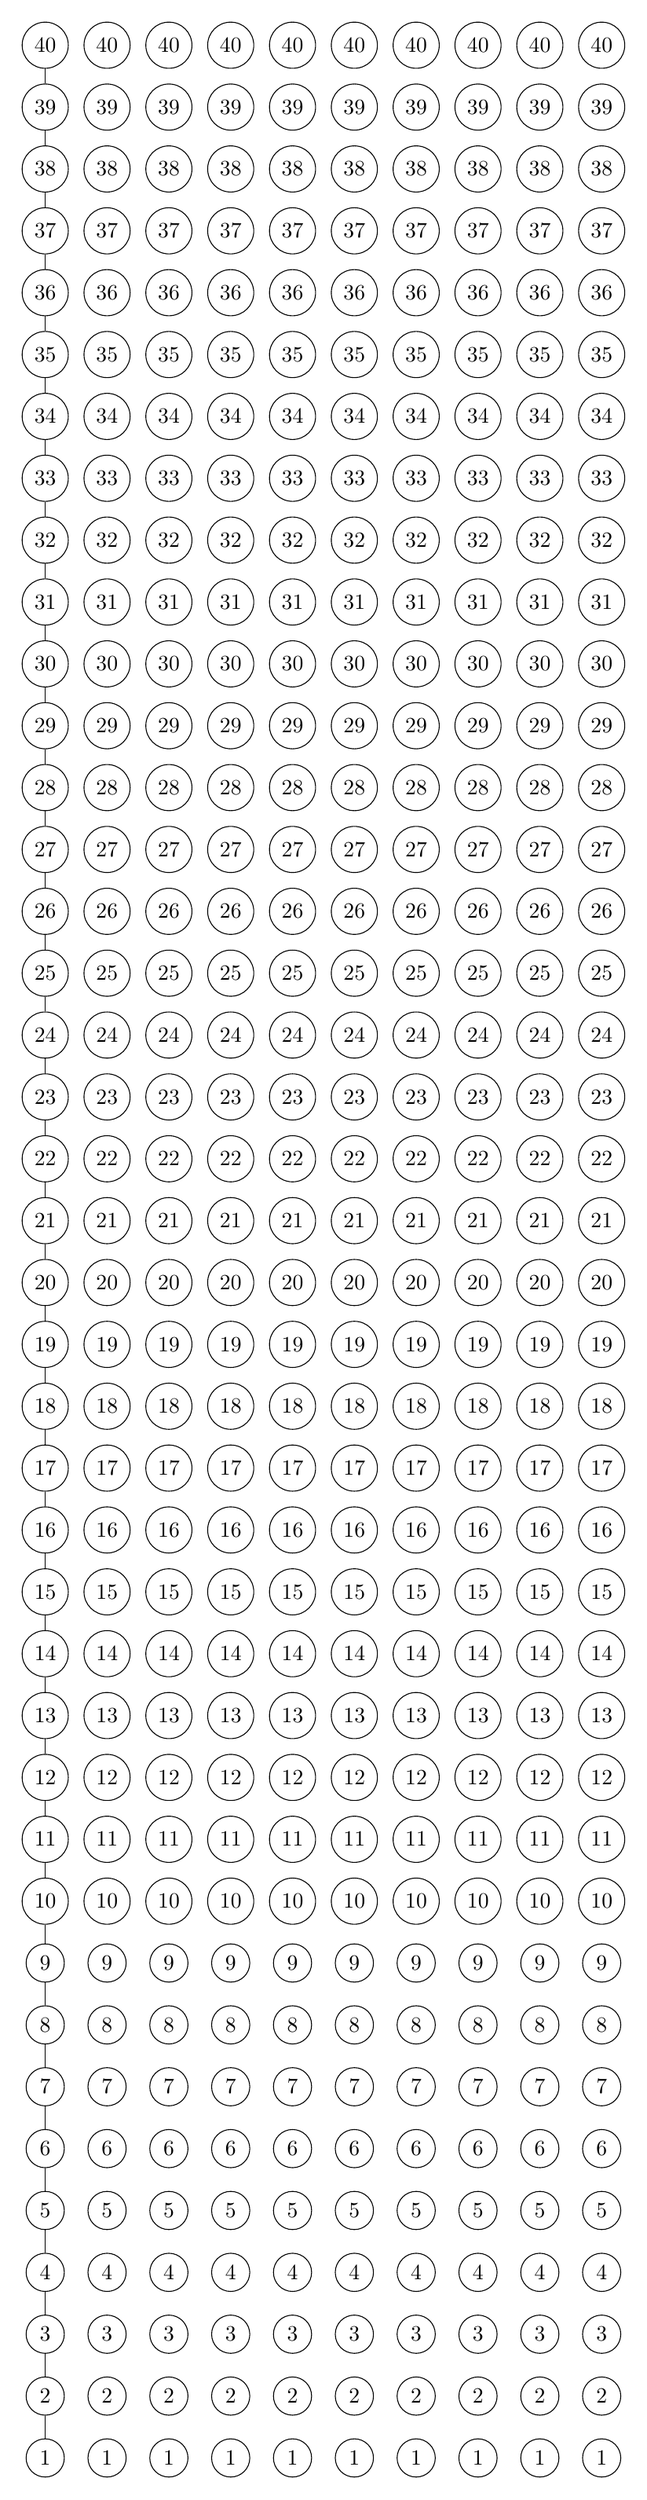
\begin{tikzpicture}
\foreach \i in {1,...,40} {
  \foreach \j in {1,...,10} {
    \node[draw, circle] (n\i-\j) at (\j,\i) {\i};
  }
}
\foreach \i in {1,...,39} { \draw (n\i-1) -- (n\the\numexpr\i+1\relax-1); }
\end{tikzpicture}
\end{document}
